\chapter{Peak Demand Management}
\label{chp:pdm}

\glsresetall

%\section{Background}
%\label{pdm:background}

\section{Summary}

Large electricity consumers pay a \textit{\acrlong{NPDC}} in addition to their actual electrical consumption per day. Reducing peak demand can yield significant savings for Monash University. 
One way to reduce peak demand without changing existing consumption patterns is to use batteries. We can minimise the peak demand and therefore the \acrlong{NPDC} by fully charging batteries before peak times and fully discharging them at peak times. To achieve this goal, this work develops a method that combines \acrlong{LP} and \acrlong{RHRS} to automatically schedule batteries based on demand forecasts. The results show that by using the existing \acrlong{VFB} and \acrlong{Liionb}, we can reduce the annual \acrlong{NPDC} of Monash Clayton campus by 2\% at most and the monthly \acrlong{NPDC} by 13\% at most for 2020. 
 
\section{Peak Demand Tariff}
\label{pdm:tariff}

Large electricity consumers, such as a customer, a company or a premier with 400 MWh electrical consumption per year, pay a \textit{\gls{NPDC}} in addition to their actual electrical consumption per day. For the Clayton campus of Monash University, this \gls{NPDC} includes two (2) components: \\

\begin{itemize}
	\item An annual maximum demand component: This component is calculated based on the maximum average demand in 30 minutes on a rolling 12-month basis. This rolling 12-month period is defined as the 11 full calendar months prior to the current day and the current month. Particularly, this component is applied to 30-minute intervals from 7am to 7pm on Monash work days. The tariff for this component is \$131.7 / MVA per day, which is about \$48k per MVA per year. The definition of Monash work days is provided in Section~\ref{prob:input:tariff}. 
	
	\item A monthly maximum demand component for summer months: This component is calculated based on the maximum average demand in 30 minutes for each full calendar month over the five summer periods from 1 Nov to 31 Mar. Particularly, this component is applied to 30-minute intervals from 3pm to 6pm on Monash work days during the five summer months. The tariff for this component is \$162.5 / MVA per day, which is in total \$24.5k per MVA per five-summer-month. 
\end{itemize} 
The tariffs for the \gls{NPDC} vary annually. However, in recent years, the changes are within plus or minus 5---10\% of the above numbers. 
Reducing peak demand can yield significant savings for Monash University. Imagine a scenario where 1 MVA is reduced from the highest average demand in a 30-minute interval, it will yield approximately \$72000  or up to \$ 144 / MWh, which is roughly ten times of the maximum wholesale price cap for electrical consumption, or a thousand times of retail electricity rates.


\section{Methodology of Battery Scheduling for Peak Demand Management}

One way to reduce peak demand effectively without changing existing consumption patterns is to use \glspl{battery}. 
We can minimise the \gls{NPDC} by fulling charging \glspl{battery} during off-peak times and discharging them at peak times. 
%We can charge \glspl{battery} during off-peak times and discharge them at peak times to reduce peak demand. Particularly, we can reduce peak demand as much as possible by ensuring \glspl{battery} are fully charged before the peak demand intervals and fully discharging \glspl{battery} during those intervals to minimise the \gls{NPDC}. 
The minimisation of the \gls{NPDC} using \glspl{battery} can be achieved by computer algorithms that predict future demands based on historic demands, and plan battery operations in advance in order to charge and discharge \glspl{battery} at the best times. This work is interested in such algorithms.
This work follows the methodology explained in Section~\ref{intro:methodology} to optimally schedule batteries and incorporate uncertainty in demand forecasts, using \textit{\glsfirst{LP}} models and the \textit{\glsfirst{RHRS}}. 

%The algorithms developed in this work follows the methodology introduction in Section~\ref{intro:methodology}, which is combing \textit{\glsfirst{LP}} models and \textit{\glsfirst{RHRS}} to optimally schedule batteries and incorporate uncertainty in the demand forecasts. 

%\subsection{Chapter Structure}
%
%This chapter presents the development of the battery scheduling algorithm for peak demands management as follows: 
%\begin{itemize}
%	\item Section~\ref{pdm:prob} presents the mathematical notations and formulation of the battery scheduling problem for peak demand management. 
%	
%	\item Section~\ref{pdm:method} introduces the \gls{LP} model for solving the battery scheduling problem and the \gls{RHRS} for incorporating uncertainty in demand forecasts. 
%	
%	\item Section~\ref{pdm:exp}:
%	
%	\item Section~\ref{pdm:conclusion}:
%	
%\end{itemize}

\section{Battery Scheduling Problem for Peak Demand Management}
\label{pdm:prob}

This work studies a battery scheduling problem where batteries are scheduled to minimise the \glsfirst{NPDC} given the annual peak demand tariff, the monthly peak demand tariff for summer months, demand forecasts and historic demands. 
This section presents the input parameters, variables, constraints, objective functions and mathematical formulation of the battery scheduling problem. 


%The \gls{PDMP} is concerned with scheduling batteries to minimise the peak demand charges for the yearly maximum demand and the summer peak demand. This section presents the problem model including the parameters, variables, constraints and objective functions. 

\subsection{Problem Parameters}

The input parameters for this battery scheduling problem include time intervals, battery specifications, peak demand tariffs and applicable hours, pre-defined demand thresholds, demand forecasts and historic demands.

\subsubsection{Time Interval}

A day is considered as a finite number of time intervals for scheduling. 
%At the time of this work, the wholesale electricity price is provided by \gls{AEMO} for every thirty minutes. Therefore, this work divides a day into 48 thirty-minute intervals for scheduling batteries. 
We assume that the charge or discharge rate of a battery does not change in a time interval. Let us write:

\begin{itemize}
	\item \gls{T} as the length in minutes of each time interval,
	
	\item $\gls{N^day} = 1440 / \gls{T}$ as the total number of time intervals per day,
	
	\item $\gls{N^hour} = 60 / \gls{T} $ as the total number of time intervals per hour,
	
	%	\item \gls{n} as the index of a time interval.
\end{itemize}
We have chosen $\gls{T} = 30 $ mins for this work, because at the time of this work, the wholesale electricity prices were updated every thirty minutes. 

\subsubsection{Battery Specification}

The total number of batteries is denoted as \gls{N^battery}. Each battery $i \in [1, \gls{N^battery}]$ is modelled by the following elements:

\begin{itemize}
	\item \gls{init_energy}: the initial energy level at the beginning of the day (in kWh)
	
	\item \gls{min_cap}: the minimum allowed energy capacity (in kWh)
	
	\item \gls{max_cap}: the maximum allowed energy capacity (in kWh)
	
	\item \gls{max_power}: the maximum power rate (in kW)
	
	\item \gls{ch_bn}: the amount of power charged to the battery at time interval $n$ (in kW): 
	
	\item \gls{disch_bn}: the amount of power discharged from the battery at time interval $n$ (in kW) 
	
	\item \gls{rte}: the round-trip efficiency (between 0 and 1)
	
	\item \gls{soc_n}: a \gls{SOC} profile --- the amount of energy remaining in the battery at time interval $n$ (in kWh)
\end{itemize}


\subsubsection{Peak Demand Tariff and Applicable Hour}
\label{prob:input:tariff}

The peak demand tariffs include two components:

\begin{itemize}
	\item The annual maximum demand component: \gls{annual_charge} = \$131.7 / MVA.
	
	\item The summer monthly component: \gls{summer_charge} = \$ 162.5 / MVA. 
	
\end{itemize}
%This work simplifies the conversion between MVA and MW by allowing 1 MVA = 1 MW. 
Although the \gls{NPDC} is calculated in MVA, in the Monash context, MW can be used as proxy, due to persistent near unity Power Factor (typically at 0.98 or 0.99). Furthermore, the \$ / MVA based charge applies to 1/2 hour with the highest MW's. For example, the selection criteria for the peak is unchanged between MVA, on the basis of the charge (\$ / MVA) differs by 1 - 2 \%. 1 MVA = 1 MW / Power Factor. 

Note that both tariffs are applied to Monash work days, which are defined in \url{https://www.monash.edu/students/admin/dates/holidays}.
We have also introduced binary variables to indicate the hours that a tariff is applied to:
\begin{itemize}
	\item The hours to which the annual maximum demand tariff is applied: \\
	$\gls{annual_charge_times} = \{ \glssymbol{annual_charge_times} = 1~ if ~ 7 \times 2 - 1 \leq n \leq 19 \times 2 ~ else~ 0~ \vert ~ n \in [1,\gls{N^day}] \}$.
	
	\item The hours to which the monthly maximum demand tariff is applied: \\
	$\gls{summer_charge_times} = \{ \glssymbol{summer_charge_times} = 1 ~ if ~ 15 \times 2 - 1 \leq n \leq 18 \times 2~  else~  0 ~ \vert ~ n \in [1,\gls{N^day}]\} $.
	
\end{itemize}

We have also considered a pre-defined maximum demand threshold for each tariff:
\begin{itemize}
	\item The pre-defined maximum demand threshold for the annual maximum demand tariff: \gls{annual_peak_previous}.
	
	\item The pre-defined maximum demand threshold for the monthly maximum demand tariff:
	\gls{summer_peak_previous}. 
\end{itemize}
These two pre-defined maximum demand thresholds can be given by users or calculated from historic demands. 

\subsubsection{Demand Forecast}

Demand forecasts are required to plan the battery operations in advance. 
At the time of this work, at each time interval $n$, the demand is forecasted from the upcoming time interval $n+1$ until 6pm of the same day.  However, to allow batteries to charge after 6pm, we assume the forecasted demand after 6pm is zero. Let us write \gls{demand} as the demand per time interval in kW. 

%The load data required for this work is the load forecast \gls{load} for each time step $n$ (in kWh). 

\subsection{Historic Demand}

Historic demands are used to calculated the maximum demands in order to calculate the \gls{NPDC}. Ideally, at each time interval $n$, the historic demands should be for the 12 months prior to the current time interval. If less than 12 months of data is provided, the maximum demands for peak demand tariffs will be calculated from the available data. Let us write the historic demands at time interval $n$ as \gls{historic_demand_n}.


\subsection{Problem Variables}

The decision variables include the amount of power charged to or discharged from each battery at each time interval: \gls{ch_bn} and \gls{disch_bn}.
Other variables include:
\begin{itemize}
	\item The modified demand per time interval \gls{demand'}, calculated as Equation~\ref{equ:modify_demand}.
	
	\begin{equation}
		\label{equ:modify_demand}
		\forall n \in [1, \gls{N^day}], ~ \gls{demand'} = \gls{demand} +\sum_{i=1}^{\gls{N^battery}} ( \gls{ch_bn} + \gls{disch_bn} )
	\end{equation}
	
	\item The maximum demand in the hours that the annual peak demand tariff is applied to \gls{annual_peak},  computed as Equation~\ref{equ:max-demand-annual} and~\ref{equ:max-demand-annual2}.
	
	\begin{equation}
		\label{equ:max-demand-annual}
		\forall n \in [1, \gls{N^day}], ~ \gls{annual_peak} \geq \gls{demand'} \times \glssymbol{annual_charge_times}
	\end{equation}
	
	\begin{equation}
		\label{equ:max-demand-annual2}
		\gls{annual_peak} \geq \gls{annual_peak_previous}
	\end{equation}
	
	\item The maximum demand in the hours that the summer monthly tariff is applied to \gls{summer_peak}, calculated as Equation~\ref{equ:max-demand-summer} and~Equation~\ref{equ:max-demand-summer2}.
	
	\begin{equation}
		\label{equ:max-demand-summer}
		\forall n \in [1, \gls{N^day}], ~ \gls{summer_peak} \geq \gls{demand'} \times \glssymbol{summer_charge_times}
	\end{equation}
	
	\begin{equation}
		\label{equ:max-demand-summer2}
		\gls{summer_peak} \geq \gls{summer_peak_previous}
	\end{equation}
	
\end{itemize}


\subsection{Problem Constraints}
\label{pdm:problem:contraints}

Each battery $b$ has the following constraints:

\begin{itemize}
	\item \textit{Charge or discharge only constraint}: At each time interval $n$, each battery can either charge or discharge, described as Equation~\ref{constraint:either-charge-discharge}.
	%	
	\begin{equation}
		\label{constraint:either-charge-discharge}
		\forall i \in [1, \gls{N^battery}], ~ \forall n \in [1, \gls{N^day}],~ \gls{ch_bn} \times \gls{disch_bn} = 0
	\end{equation}
	
	\item \textit{Maximum power constraint}: At each time interval $n$, each battery cannot charge or discharge at a rate higher than the maximum power rate, defined as Equation~\ref{constraint:max-charge} and~\ref{constraint:max-discharge}.
	
	\begin{equation}
		\label{constraint:max-charge}
		\forall i \in [1, \gls{N^battery}], ~ \forall n \in [1, \gls{N^day}],~ 0 \leq \gls{ch_bn} \leq \gls{max_power}
	\end{equation}
	
	\begin{equation}
		\label{constraint:max-discharge}
		\forall i \in [1, \gls{N^battery}], ~ \forall n \in [1, \gls{N^day}],~ 0 \leq -\gls{disch_bn} \leq \gls{max_power}
	\end{equation}
	
	\item \textit{Maximum-minimum capacity constraint}: At each time interval $n$, each battery cannot have more (or less) than the maximum (or the minimum) allowed energy, described as Equation~\ref{constraint:min-max-cap}.
	
	\begin{equation}
		\label{constraint:min-max-cap}
		\forall i \in [1, \gls{N^battery}], ~ \forall n \in [1, \gls{N^day}],~ \gls{min_cap} \leq \gls{soc_n} \leq \gls{max_cap}
	\end{equation}
	
	\item \textit{\gls{SOC} constraints}: At the first time interval of the scheduling horizon, each battery must satisfy an initial energy level, defined as Equation~\ref{constraint:init-energy} and~\ref{constraint:soc}.
	
	\begin{equation}
		\label{constraint:init-energy}
		\forall i \in [1, \gls{N^battery}], ~(\glssymbol{soc_n} \text{}_1 - \gls{init_energy}) \times \gls{N^hour} = \glssymbol{ch_bn} \text{}_1 \times \gls{rte} + \glssymbol{disch_bn} \text{}_1
	\end{equation}
	At each time interval $n$, the \gls{SOC} depends on the \gls{SOC} at time interval $n-1$, and the charge and discharge at time interval $n$:
	
	\begin{equation}
		\label{constraint:soc}
		\forall i \in [1, \gls{N^battery}], ~\forall n \in [2, \gls{N^day}], ~ (\glssymbol{soc_n} \text{}_n - \glssymbol{soc_n} \text{}_{n-1} ) \times \gls{N^hour} = \gls{ch_bn} \times \gls{rte} + \gls{disch_bn}
	\end{equation}
	
	
	%	 \item \textit{Maximum demand constraint}: This maximum demand constraint is introduced to calculate the maximum demand from the modified demand per time interval, described as Equation~
	%	 
	%	\begin{Equation}
		%		\forall 
		%	\end{Equation}
	
\end{itemize}

Note that, there are various ways to apply round-trip efficiencies when calculating \glspl{SOC}. For example, some works divided actual charges by the efficiency and multiplied discharges with the efficiency~\cite{Couraud2020, Maheshwari2020}. Some works multiplied both charges and discharges with the efficiency~\cite{Adika2014}, instead. Some other works multiplied charges with the efficiency and divided discharges by the efficiency~\cite{Pandzic2019,GonzalezCastellanos2020}. This work chooses to multiple charges with the efficiency only as shown in Equation~\ref{constraint:init-energy} and~\ref{constraint:soc}. However, the use of efficiencies can be changed according to actual needs for different problem instances.  


\subsection{Problem Objectives}
\label{pdm:problem:objectives}
The objectives of our battery scheduling problem for peak demand management include minimisation of the peak demand charge, a penalty cost of charging or discharging batteries frequently and a penalty cost of not fully charging the battery before the end of the day. Each objective is calculated as follows: 

\begin{itemize}
	\item Peak demand charge \gls{f_charge}: 
	
	\begin{equation}
		\gls{f_charge} =  \gls{annual_peak} \times \gls{annual_charge} + \gls{summer_peak} \times \gls{summer_charge} \times \alpha
	\end{equation}
	
	\begin{equation}
		\alpha = 
		\begin{cases}
			1,				& \text{if the current month is Nov/Dec/Jan/Feb/March, } \\
			%		& \text{and the current time is between 3pm to 6pm}     \\
			0,              & \text{otherwise}
		\end{cases}
	\end{equation}
	
	
	\item Penalty cost of frequent charging or discharging \gls{g_battery}:
	
	\begin{equation}
		\gls{g_battery} = \sum_{i=1}^{\gls{N^battery}}\sum_{n=1}^{\gls{N^day}} \gls{ch_bn} 
	\end{equation}
	%todo: literature??
	
	\item Penalty cost of not fully charging \glspl{battery} before the end of the day \gls{g_eod}:
	
	\begin{equation}
		\gls{g_eod} = \sum_{i=1}^{\gls{N^battery}} ( \gls{max_cap} -  \glssymbol{soc_n}_{ \gls{n^eod}  })
	\end{equation}
	where  \gls{n^eod} is the last time interval of the day. 
	
	\item Combined objective \gls{h_combined}:
	
	\begin{equation}
		\gls{h_combined} = \gls{w_charge} \times \gls{f_charge} + \gls{w_penalty} \times \gls{g_battery}
	\end{equation}
	
\end{itemize}

Each objective is multiplied by a weight, denoted as follows:

\begin{itemize}
	\item The weight of the peak demand charge: \gls{w_charge}.
	
	\item The weights of the penalty costs: \gls{w_penalty} and \gls{w_eod}
\end{itemize}
The values of \gls{w_charge}, \gls{w_penalty} and \gls{w_eod} will affect the contributions of the peak demand charge and the penalty in the combined objective. This work considers \gls{w_charge} to be one. The values of \gls{w_penalty} and \gls{w_eod} were chosen based on observations from experiments. 


\subsection{Formal Problem Formulation}

The battery scheduling problem for peak demand management can be formulated as follows:
%This problem seeks the best values for the charge/discharge per time interval: \gls{ch_bn} and \gls{disch_bn} that solves the following problem:

\begin{equation*}
	\label{problem}
	\begin{aligned}
		& {\textsf{minimise}}
		& &  \gls{h_combined}   \\
		& \textsf{subject to}
		& & 
		(\ref{constraint:either-charge-discharge}), 
		~(\ref{constraint:max-charge}), 
		~(\ref{constraint:max-discharge}), 
		~(\ref{constraint:min-max-cap}), 
		~(\ref{constraint:init-energy}), 
		%		~(\ref{constraint:end-energy}), 
		~(\ref{constraint:soc})\\
	\end{aligned}
\end{equation*}
%This is an optimisation problem where the decision variables \gls{ch_bn} and \gls{disch_bn} are continuous, the constraints are xxxx and the combined objective function is linear. 

\section{Battery Scheduling Method for Peak Demand Management}
\label{pdm:method}

The solution to solving our battery scheduling problem includes a \glsfirst{LP} model implemented in a modelling language called MiniZinc~\cite{Stuckey2018}. In order to incorporate uncertainty in future demand, a \glsfirst{RHRS} is applied to update battery schedules regularly during the day based on new demand forecasts.  This section describes the \gls{LP} in Section~\ref{pdm:method:model} and the \gls{RHRS} in Section~\ref{method:rhrs}.

\subsection{Linear Programming Model for Peak Demand Management}
\label{pdm:method:model}

\begin{figure}[hp!]
	\centering
	\label{pdm:method:lp}
	\caption{\gls{LP} model for solving our battery scheduling problem for peak demand management}
	% ======== MIP model for the DSP-SH ========== %
	\begin{lstlisting}[language=minizinc,escapeinside={(*@}{@*)}]
% ---------- Input parameters ---------- % (*@\label{mzn:lp:paramStart}@*) 		
int: num_intervals; 			(*@\label{mzn:lp:num_intervals}@*)
int: num_intervals_hour;    (*@\label{mzn:lp:num_intervals_hour}@*) 
int: eod_interval; 				(*@\label{mzn:lp:eod_interval}@*) 
set of int: INTERVALS = 1..num_intervals; 
	
int: num_batteries;
set of int: BATTERIES = 1..num_batteries;			(*@\label{mzn:lp:num_batteries}@*)
array[BATTERIES] of float: init_socs;   	   (*@\label{mzn:lp:init_socs}@*)
array[BATTERIES] of float: min_socs;      (*@\label{mzn:lp:min_socs}@*)
array[BATTERIES] of float: max_socs;     (*@\label{mzn:lp:max_socs}@*)
array[BATTERIES] of float: max_powers;   	 	   (*@\label{mzn:lp:max_powers}@*)
float: power_limit = max(max_powers);			
array[BATTERIES] of float: efficiencies;				(*@\label{mzn:lp:efficiencies}@*)

array[INTERVALS] of float: forecasts;					(*@\label{mzn:lp:forecasts}@*)
float: demand_limit;
	
array[int] of float: tariff_rates;								(*@\label{mzn:lp:tariff_rates}@*)
array[int, INTERVALS] of int: tariff_times;			   (*@\label{mzn:lp:tariff_times}@*)
set of int: RATES = index_set(tariff_rates); 
array[int] of float: previous_max_demands; 		  (*@\label{mzn:lp:previous_max_demands}@*)
float: w_penalty; (*@\label{mzn:lp:w_penalty}@*) 
float: w_eod; (*@\label{mzn:lp:w_eod}@*) 	(*@\label{mzn:lp:paramEnd}@*)
	
% ---------- Variables ---------- % (*@\label{mzn:lp:varsStart}@*)
array[RATES] of var 0..demand_limit: max_demands; 				       (*@\label{mzn:lp:max_demands}@*)
array[BATTERIES, INTERVALS] of var 0..power_limit: charges;        (*@\label{mzn:lp:charges}@*)
array[BATTERIES, INTERVALS] of var -power_limit..0: discharges;  (*@\label{mzn:lp:discharges}@*)
array[BATTERIES, INTERVALS] of var float: soc;								 (*@\label{mzn:lp:socs}@*)
array[INTERVALS] of var 0..demand_limit: modified_demand = array1d([forecasts[i] + sum(b in BATTERIES)(charges[b, i] + discharges[b, i])| i in INTERVALS]);  (*@\label{mzn:lp:modified_demand}@*) (*@\label{mzn:lp:varsEnd}@*)

% ---------- Constraints ---------- %	(*@\label{mzn:lp:ctsStart}@*)
% Charge or discharge only constraint   (*@\label{mzn:lp:charge-discharge_cts}@*)
constraint forall(b in BATTERIES, i in INTERVALS) (charges[b, i] * discharges[b, i] = 0); 

% Maximum power constraints  (*@\label{mzn:lp:power_cts}@*)
constraint forall(b in BATTERIES, i in INTERVALS)(discharges[b, i] <= 0.0);
constraint forall(b in BATTERIES, i in INTERVALS)(discharges[b, i] >= -max_powers[b]);

constraint forall(b in BATTERIES, i in INTERVALS)(charges[b, i] >= 0.0);
constraint forall(b in BATTERIES, i in INTERVALS)(charges[b, i] <= max_powers[b]);		

% Maximum-minmum capacity constraints  (*@\label{mzn:lp:max-min-cap_cts}@*)
constraint forall(b in BATTERIES, i in INTERVALS)(soc[b, i] <= max_socs[b]);
constraint forall(b in BATTERIES, i in INTERVALS)(soc[b, i] >= min_socs[b]);

% SOC constraints   (*@\label{mzn:lp:soc_cts}@*)
constraint forall(b in BATTERIES) 
(soc[b, 1] * num_intervals_hour - init_socs[b] * num_intervals_hour = 
charges[b, 1] * efficiencies[b] + discharges[b, 1]);

constraint forall(b in BATTERIES, i in 2..num_intervals) 
(soc[b, i] * num_intervals_hour - soc[b, i - 1] * num_intervals_hour = 
charges[b, i] * efficiencies[b] + discharges[b, i]);

% Max demand calculation  (*@\label{mzn:lp:max-demands_cts}@*)
constraint forall(r in RATES)(max_demands[r] >= previous_max_demands[r]);
constraint forall(r in RATES, i in INTERVALS)
(max_demands[r] >= modified_demand[i] * tariff_times[r, i]); (*@\label{mzn:lp:ctsEnd}@*)

% ---------- Objectives ---------- % (*@\label{mzn:lp:objStart}@*)
var float: eod_penalty = sum(i in INTERVALS, r in RATES, b in BATTERIES) ((max_socs[b] - soc[b, i]) * (1 - charge_times[r, i]));  (*@\label{mzn:lp:eod_penalty}@*)
var float: penalty = sum(b in BATTERIES, i in INTERVALS)(charges[b, i]); (*@\label{mzn:lp:penalty}@*)
var float: costs = sum(r in RATES) (max_demands[r] * tariff_rates[r]); (*@\label{mzn:lp:costs}@*)
var float: combined_obj = costs + penalty * w_penalty + eod_penalty * w_eod; (*@\label{mzn:lp:combined_obj}@*) (*@\label{mzn:lp:objEnd}@*)
solve minimize combined_obj;
\end{lstlisting}
\end{figure}

Figure~\ref{pdm:method:lp} shows the \gls{LP} model for solving the battery scheduling problem.
We declare the input parameters from Line~\ref{mzn:lp:paramStart} to~\ref{mzn:lp:paramEnd}, including:
\begin{itemize}
	\item The number of time intervals per day: \mzninline|num_intervals|, line~\ref{mzn:lp:num_intervals},
	
	\item The number of time intervals per hour: \mzninline|num_intervals_hour|, line~\ref{mzn:lp:num_intervals_hour},
	
	\item The index of the last time interval of the day: \mzninline|eod_interval|, line~\ref{mzn:lp:eod_interval},
	
	\item The number of batteries: \mzninline|num_batteries|, line~\ref{mzn:lp:num_batteries},
	
	\item The initial \glspl{SOC} or energy levels: \mzninline|init_socs|, line~\ref{mzn:lp:init_socs},
	
	\item The minimum \glspl{SOC} or capacities: \mzninline|min_socs|, line~\ref{mzn:lp:min_socs},
	
	\item The maximum \glspl{SOC} or capacities: \mzninline|max_socs|, line~\ref{mzn:lp:max_socs},
	
	\item The maximum power rates: \mzninline|max_powers|, line~\ref{mzn:lp:max_powers},
	
	\item The battery efficiencies: \mzninline|efficiencies|, line~\ref{mzn:lp:efficiencies},
	
	\item The demand forecasts: \mzninline|forecasts|, line~\ref{mzn:lp:forecasts},
	
	\item The peak demand tariff rates: \mzninline|tariff_rates|, line~\ref{mzn:lp:tariff_rates},
	
	\item The applicable hours or times of tariffs: \mzninline|tariff_times|, line~\ref{mzn:lp:tariff_times},
	
	\item The pre-defined maximum demand thresholds for tariffs (given by users or calculated from historic demands): \mzninline|previous_max_demands|, line~\ref{mzn:lp:previous_max_demands},
	
	\item The weight for the penalty cost of charging/discharging \glspl{battery} frequently: \mzninline|w_penalty|, line~\ref{mzn:lp:w_penalty}.
	
	\item The weight of the penalty cost of not fully charging \glspl{battery} before the end of the day: \mzninline|w_eod|, line~\ref{mzn:lp:w_eod}.
\end{itemize}

We introduce the variables from line~\ref{mzn:lp:varsStart} to line~\ref{mzn:lp:varsEnd}, including:
\begin{itemize}
	\item The maximum demand for each tariff: \mzninline|max_demands|, line~\ref{mzn:lp:max_demands}.
	
	\item The amount of power charged to each battery per time interval: \mzninline|charges|, line~\ref{mzn:lp:charges}.
	
	\item The amount of power discharged from each battery per time interval: \mzninline|discharges|, line~\ref{mzn:lp:discharges}.
	
	\item The \gls{SOC} of each battery per time interval: \mzninline|socs|, line~\ref{mzn:lp:socs}.
	
	\item The modified demand per time interval: \mzninline|modified_demand|, line~\ref{mzn:lp:modified_demand}.
\end{itemize}

We define the constraints from line~\ref{mzn:lp:ctsStart} to line~\ref{mzn:lp:ctsEnd}, including:
\begin{itemize}
	\item The \textit{charge or discharge only constraint}: line~\ref{mzn:lp:charge-discharge_cts}.
	
	\item The \textit{maximum power constraint}: line~\ref{mzn:lp:power_cts}.
	
	\item The \textit{maximum-minimum capacity constraint}: line~\ref{mzn:lp:max-min-cap_cts}.
	
	\item The \textit{\gls{SOC} constraints}: line~\ref{mzn:lp:soc_cts}.
	
	\item The \textit{maximum demand constraints} for calculating the maximum demand for each peak demand tariff: line~\ref{mzn:lp:max-demands_cts}.
\end{itemize}

We specify the objective functions from line~\ref{mzn:lp:objStart} to line~\ref{mzn:lp:objEnd}, including:
\begin{itemize}
	
	\item The penalty cost of not fully charging \glspl{battery} before the end of the day: \mzninline|eod_penalty|, line~\ref{mzn:lp:eod_penalty}.
	
	\item The penalty cost of charging/discharging \glspl{battery} frequently: \mzninline|penalty|, line~\ref{mzn:lp:penalty}.
	
	\item The total peak demand charges: \mzninline|costs|, line~\ref{mzn:lp:costs}.
	
	\item The combined objective: \mzninline|combined_obj|, line~\ref{mzn:lp:combined_obj}.
\end{itemize}

\subsection{Rolling Horizon Rescheduling Strategy}
\label{method:rhrs}

The \gls{RHRS} is a method that incorporates uncertainty in demand forecasts. This strategy applies the optimal solution to an optimisation problem for a period of time, after which the values of the input parameters are updated and new optimal solution is obtained~\cite{Marietta2014}. More specifically, this strategy solves a problem in an iterative manner as follows:

\begin{enumerate}
	\item At any time interval of the day $n$, the battery scheduling problem is solved for the entire scheduling horizon, which can be from the current time interval until the last time interval of the day, or the next 24 hours. \label{method:rhrs:solve}
	
	\item Use the optimal decisions for time intervals $n$, $n + 1$, ..., $n + x$ to control the batteries. \label{method:rhrs:apply}
	
	\item At time interval $n + x$, the battery scheduling problem is solved again for the entire scheduling horizon, and Step~\ref{method:rhrs:solve} and Step~\ref{method:rhrs:apply} are repeated every $x$ intervals until the last time interval of the day. 
\end{enumerate}
This iterative process can be illustrated as Figure~\ref{fig:rolling-horizon}.
At each iteration, the maximum demand for each tariff calculated in the previous iteration will be used as the pre-defined maximum demand thresholds for the current iteration. If the forecast maximum demand is lower than the pre-defined maximum demand thresholds at any time interval or iteration, the battery scheduling problem does not need to be solved again for that iteration. 

\begin{figure}[tbh]
	\centering
	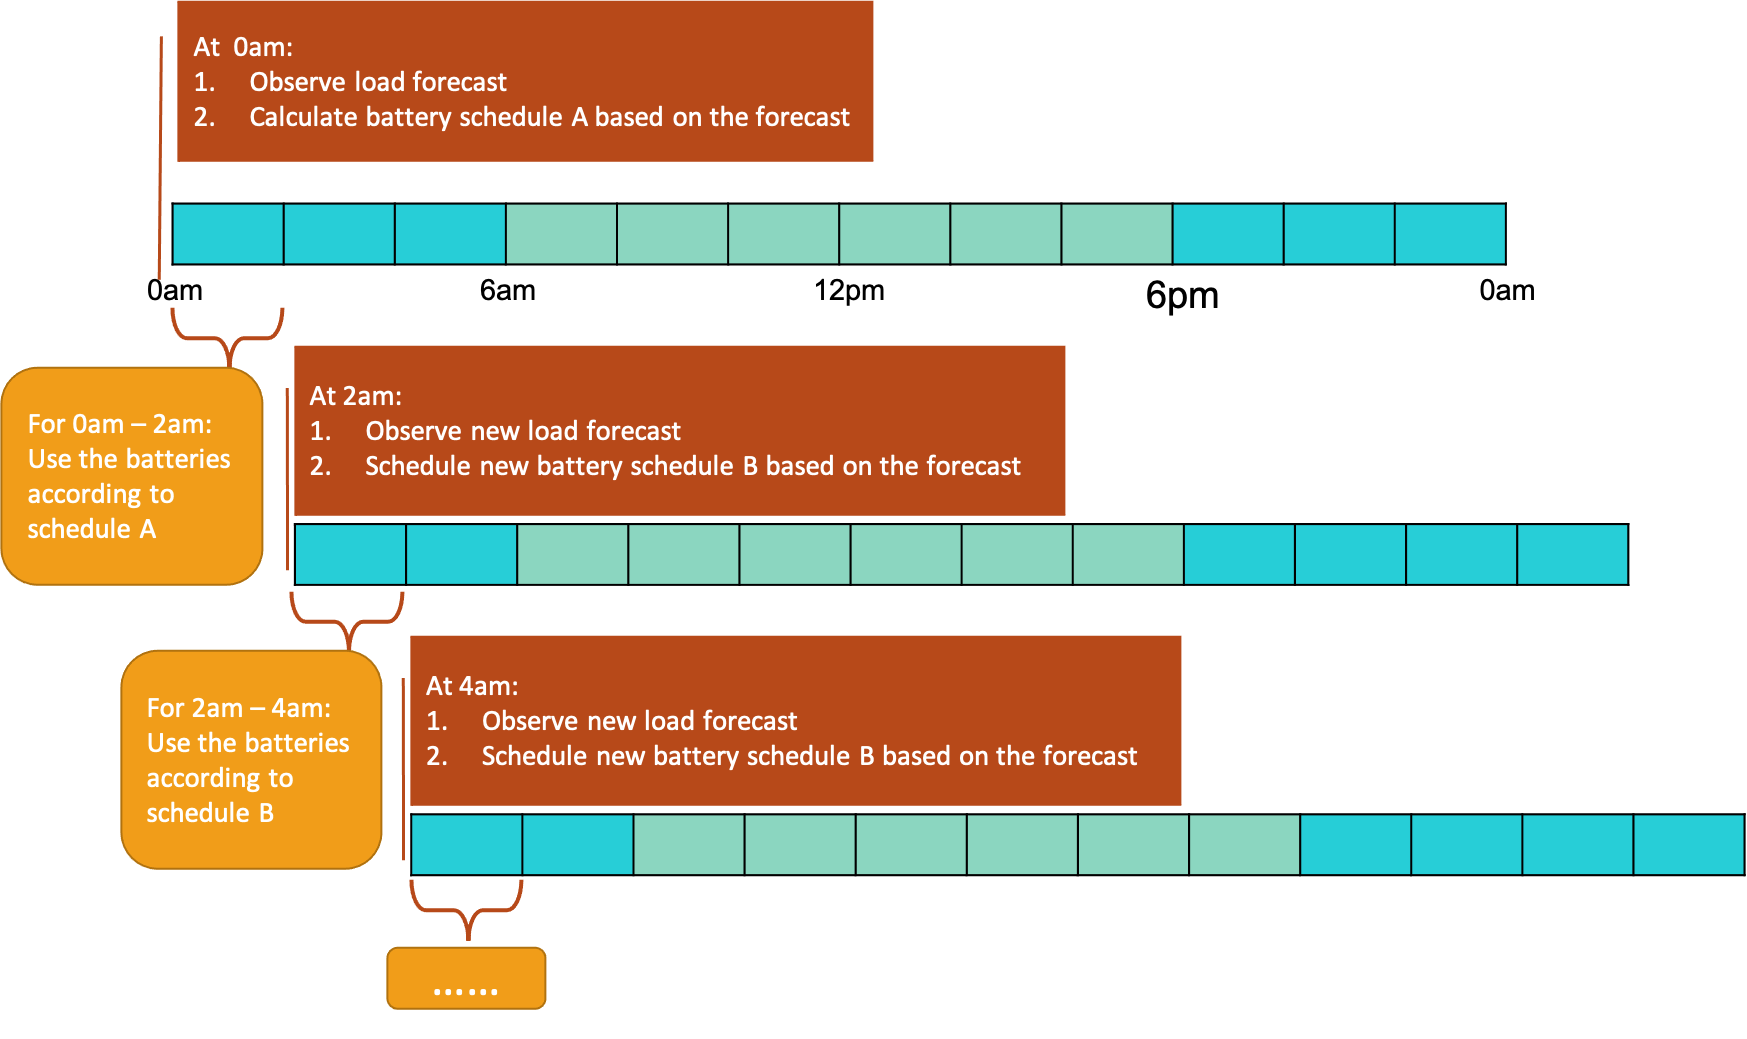
\includegraphics[width=1\linewidth]{rolling-horizon}
	\caption{Rolling horizon rescheduling strategy}
	\label{fig:rolling-horizon}
\end{figure}


%\begin{algorithm}[tbh]
%	\caption{\Acrlong{RHRS} with the \gls{LP} model}
%	\label{single:alg:ogs} 
%	\begin{algorithmic}[1]
%
%		\Require Peak demand tariffs, historic demands of the past 12 months, demand forecast for the rest of the day, battery specifications, and the frequency of updating forecasts. 
%		
%		\State At time interval $n$, schedule batteries using the \gls{LP} model based on the demand forecast.
%		
%		\State Implement the battery schedule from interval $n$ to the interval $n$ + 30 minutes/an hour/$x$ hours when the demand forecast is updated again. 
%	
%		\Ensure scheduled/actual start times of 
%	\end{algorithmic}
%\end{algorithm}




\section{Experimental Results of Battery Scheduling Method for Peak Demand Management}
\label{pdm:exp}

This section presents the experiment environments, steps and results that demonstrate the effectiveness of our battery scheduling method for peak demand management. 

\subsection{Experiment Environment}

The \glsfirst{LP} model was implemented in MiniZinc~\cite{Stuckey2018}, which is an optimisation language accepted by well-known optimisation solvers, including Gurobi and CPLEX. The \glsfirst{RHRS} was programmed in Python. Details of the implementation can be found at \url{https://bitbucket.org/dorahee2/battery-scheduling/src/master/}. The instruction of using this algorithm has been explained a wiki at \url{https://bitbucket.org/dorahee2/battery-scheduling/wiki/Home}. 
At the current stage of the project, this repository needs to remain private. Please email \texttt{dora.he3@monash.edu} for access to this repository and the wiki.

\subsection{Experiment Data}

The data for testing the battery scheduling method for peak demand management includes:

\begin{itemize}
	\item Peak demand tariffs, which have described in Section~\ref{pdm:tariff}.
	
	\item Battery details: Two batteries are used in this work.
	\begin{itemize}
		\item  A \gls{Liionb} whose maximum power rate is 120 kW, the maximum capacity is 134 kWh, and the round-trip efficiency is between 85\% and 88\%. We have chosen 88\% as the efficiency for our experiments. 
		
		\item A \gls{VFB} whose maximum power rate is 180 kW, the maximum capacity is 900 kWh and the round-trip efficiency is between 60\% and 65\%. We have chosen 65\% as the efficiency for our experiments. 
	\end{itemize}

	\item Historic demands are averaged demands at 30-minute intervals from 1st January 2020 00:00 to 31st December 2020 23:00.

	\item Demand forecasts are produced at every 30-minute interval from 1st January 2020 00:00 to 31st December 2020 23:00. Each forecast has the predicted average load for every 30-minute interval in the next 24 hours. 
	
\end{itemize}

At the time of this work, the forecast results from Farshid's model were not available for testing. Frits has developed a naive machine learning model to forecast demands for these experiments. 
In practise, demand forecasts from any machine learning model can be used. 

The details of the input data including the expected values and formats of these data are explained in
\url{https://bitbucket.org/dorahee2/battery-scheduling/wiki/Peak\%20demand\%20management/2.\%20Input\%20data}. 

\subsection{Experiment Results}

We have tested the effectiveness of our battery scheduling method for peak demand management using the data from 1 Jan 2020 to 30 Dec 2020 in the following step:

\begin{enumerate}
	\item Set the time window to be from 6am to 0am on 1 Jan 2020. 
	
	\item Read the demand forecast of this time window and schedule batteries for this time window based on the forecast. \label{pdm:exp:step2}
	
	\item Select the frequency at which the forecast is updated, such as every 24/12/6/3 hours or 30 minutes.
	
	\item Apply the optimised battery schedule for the duration of the frequency. For example, add the battery charges and discharges to the actual demands for the rest of the day, or for the next 12/6/3 hours or 30 minutes.
	
	\item Move the time window for the frequency length. For example, move the time window to start from the next day, or from 12/6/3 hours or 30 minutes after 6am.  \label{pdm:exp:step5}
	
	\item Repeat Step~\ref{pdm:exp:step2} -- Step~\ref{pdm:exp:step5} at the chosen frequency until the time window reaches the last time interval on 30 Dec 2020. 
	
\end{enumerate}
Note that, in this work, the time window always starts from a time interval in a day and finishes at the last time interval of the same day. The size of the time window reduces gradually during the day and resets in the next day. However, in practice, this time window can maintain a fixed size. For example, the size of the time window can remain 24 hours.

We have scheduled \glspl{battery} using data from 1 Jan 2020 to 30 Dec 2020 and evaluated results using different forecasts and forecasting frequencies, as follows:
\begin{enumerate}
	\item Perfect forecast scenario: Using historic demands as the demand forecasts. 
	
	\item Forecasts updated every day scenario: Using the naive demand forecast model and updating the forecast once at the beginning of the day. 
	
	\item Forecast updated every 12 hours: Using the naive demand forecast model and updating the forecast every 12 hours. 
	
	\item Forecast updated every 6 hours: Using the naive demand forecast model and updating the forecast every 6 hours. 
	
	\item Forecast updated every 3 hours: Using the naive demand forecast model and updating the forecast every 3 hours. 
	
	\item Forecast updated every 30 minutes: Using the naive demand forecast model and updating the forecast every 30 minutes. 
\end{enumerate}

We have illustrated the forecast demands, the actual demands, the maximum demand associated with the annual peak demand charge, the maximum demand associated with the summer monthly peak demand charge, the charges and discharges of each battery for January of 2020 in each scenario in Figure~\ref{fig:perfect-forecasts}, ~\ref{fig:1440min-forecasts}, ~\ref{fig:720min-forecasts}, ~\ref{fig:360min-forecasts}, ~\ref{fig:30min-forecasts}.

 We have also calculated the optimised annual and monthly peak demand charges for 2020 in each scenario, and compared them with the original charges when no \glspl{battery} are used in Table~\ref{tab:pdm:exp:costs} and~\ref{tab:pdm:exp:percent}.

The results show that the batteries discharged at the maximum power rates during peak times and recharged gradually outside those times when the demand forecasts were perfect, or the demand forecasts followed the trend of the actual demands, and therefore minimising or reducing the peak demand charges. However, the batteries may recharge at the undesired times or not discharge at the desired times when the forecasts were not accurate. In the worst case, the peak demand charges may be higher than those without using batteries. 

\subsection{Findings}

We have found that this battery scheduling method can effectively reduce the peak demand charges when demand forecasts indeed approximate actual demands. However, inaccurate demand forecasts can lead to a higher peak demand charge in the worst case. 

% Please add the following required packages to your document preamble:
% \usepackage{booktabs}
\begin{landscape}
\begin{table}[tb]
	\label{tab:pdm:exp:costs}
	\caption{The actual and optimised peak demand charges}
	\begin{tabularx}{\linewidth}
		{@{}l X X X X X X@{}}
		\toprule
%		\multicolumn{1}{l|}{}  & \multicolumn{6}{c}{\textbf{Peak demand charges}}                                                                                                                                                                   \\ 
		\multicolumn{1}{l|}{}                                    & \multicolumn{1}{c}{\textbf{Annual}} & \multicolumn{1}{c}{\textbf{Jan}} & \multicolumn{1}{c}{\textbf{Feb}} & \multicolumn{1}{c}{\textbf{Mar}} & \multicolumn{1}{c}{\textbf{Nov}} & \multicolumn{1}{c}{\textbf{Dec}} \\\midrule
		\multicolumn{1}{l|}{No optimisation}                     & \$   2,212.56                       & \$   2,686.32                    & \$   2,230.80                    & \$   2,064.40                    & \$   1,758.64                    & \$   1,810.64                    \\\midrule
		\multicolumn{7}{l}{\textbf{Optimisation with forecasts}}                                                                                                                                                                                                                               \\\midrule
		\multicolumn{1}{l|}{Perfect forecasts}                   & \$   2,173.05                       & \$   2,326.61                    & \$   2,182.05                    & \$   2,015.65                    & \$   1,709.89                    & \$   1,761.89                    \\
		\multicolumn{1}{l|}{Updating forecasts every day}        & \$   2,212.56                       & \$   2,375.36                    & \$   2,230.80                    & \$   2,064.40                    & \$   1,718.39                    & \$   1,804.35                    \\
		\multicolumn{1}{l|}{Updating forecasts every 12 hours}   & \$   2,212.56                       & \$   2,375.36                    & \$   2,230.80                    & \$   2,064.40                    & \$   1,718.39                    & \$   1,804.35                    \\
		\multicolumn{1}{l|}{Updating forecasts every 6 hours}    & \$   2,212.56                       & \$   2,375.36                    & \$   2,206.95                    & \$   2,017.12                    & \$   1,729.48                    & \$   1,787.37                    \\
		\multicolumn{1}{l|}{Updating forecasts every 3 hours}    & \$   2,212.56                       & \$   2,637.57                    & \$   2,182.05                    & \$   2,017.12                    & \$   1,709.89                    & \$   1,761.89                    \\
		\multicolumn{1}{l|}{Updating forecasts every hour}       & \$   2,236.27                       & \$   2,637.57                    & \$   2,182.05                    & \$   2,015.65                    & \$   1,709.89                    & \$   1,761.89                    \\
		\multicolumn{1}{l|}{Updating forecasts every 30 minutes} & \$   2,240.23                       & \$   2,637.57                    & \$   2,182.05                    & \$   2,015.65                    & \$   1,709.89                    & \$   1,761.89                    \\ \bottomrule
	\end{tabularx}
\end{table}


\begin{table}[tb]
	\label{tab:pdm:exp:percent}
	\caption{The reductions of the optimised peak demand charges}
	\begin{tabularx}{\linewidth}
			{@{}l | X X X X X X@{}}
		\toprule
		\textbf{Forecast type}                & \textbf{Annual} & \textbf{Jan} & \textbf{Feb} & \textbf{Mar} & \textbf{Nov} & \textbf{Dec} \\ \midrule
		Perfect forecasts                     & \textbf{2\%}             & \textbf{13\%}         & 2\%          & 2\%          & 3\%          & 3\%          \\
		Updating forecasts every day          & 0\%             & 12\%         & 0\%          & 0\%          & 2\%          & 0\%          \\
		Updating forecasts every 12 hours     & 0\%             & 12\%         & 0\%          & 0\%          & 2\%          & 0\%          \\
		Updating forecasts every 6 hours      & 0\%             & 12\%         & 1\%          & 2\%          & 2\%          & 1\%          \\
		Updating forecasts every 3   hours    & 0\%             & 2\%          & 2\%          & 2\%          & 3\%          & 3\%          \\
		Updating forecasts every hour         & -1\%            & 2\%          & 2\%          & 2\%          & 3\%          & 3\%          \\
		Updating forecasts every 30   minutes & -1\%            & 2\%          & 2\%          & 2\%          & 3\%          & 3\%          \\ \bottomrule
	\end{tabularx}
\end{table}

\end{landscape}

\begin{figure}[p]
	\centering
	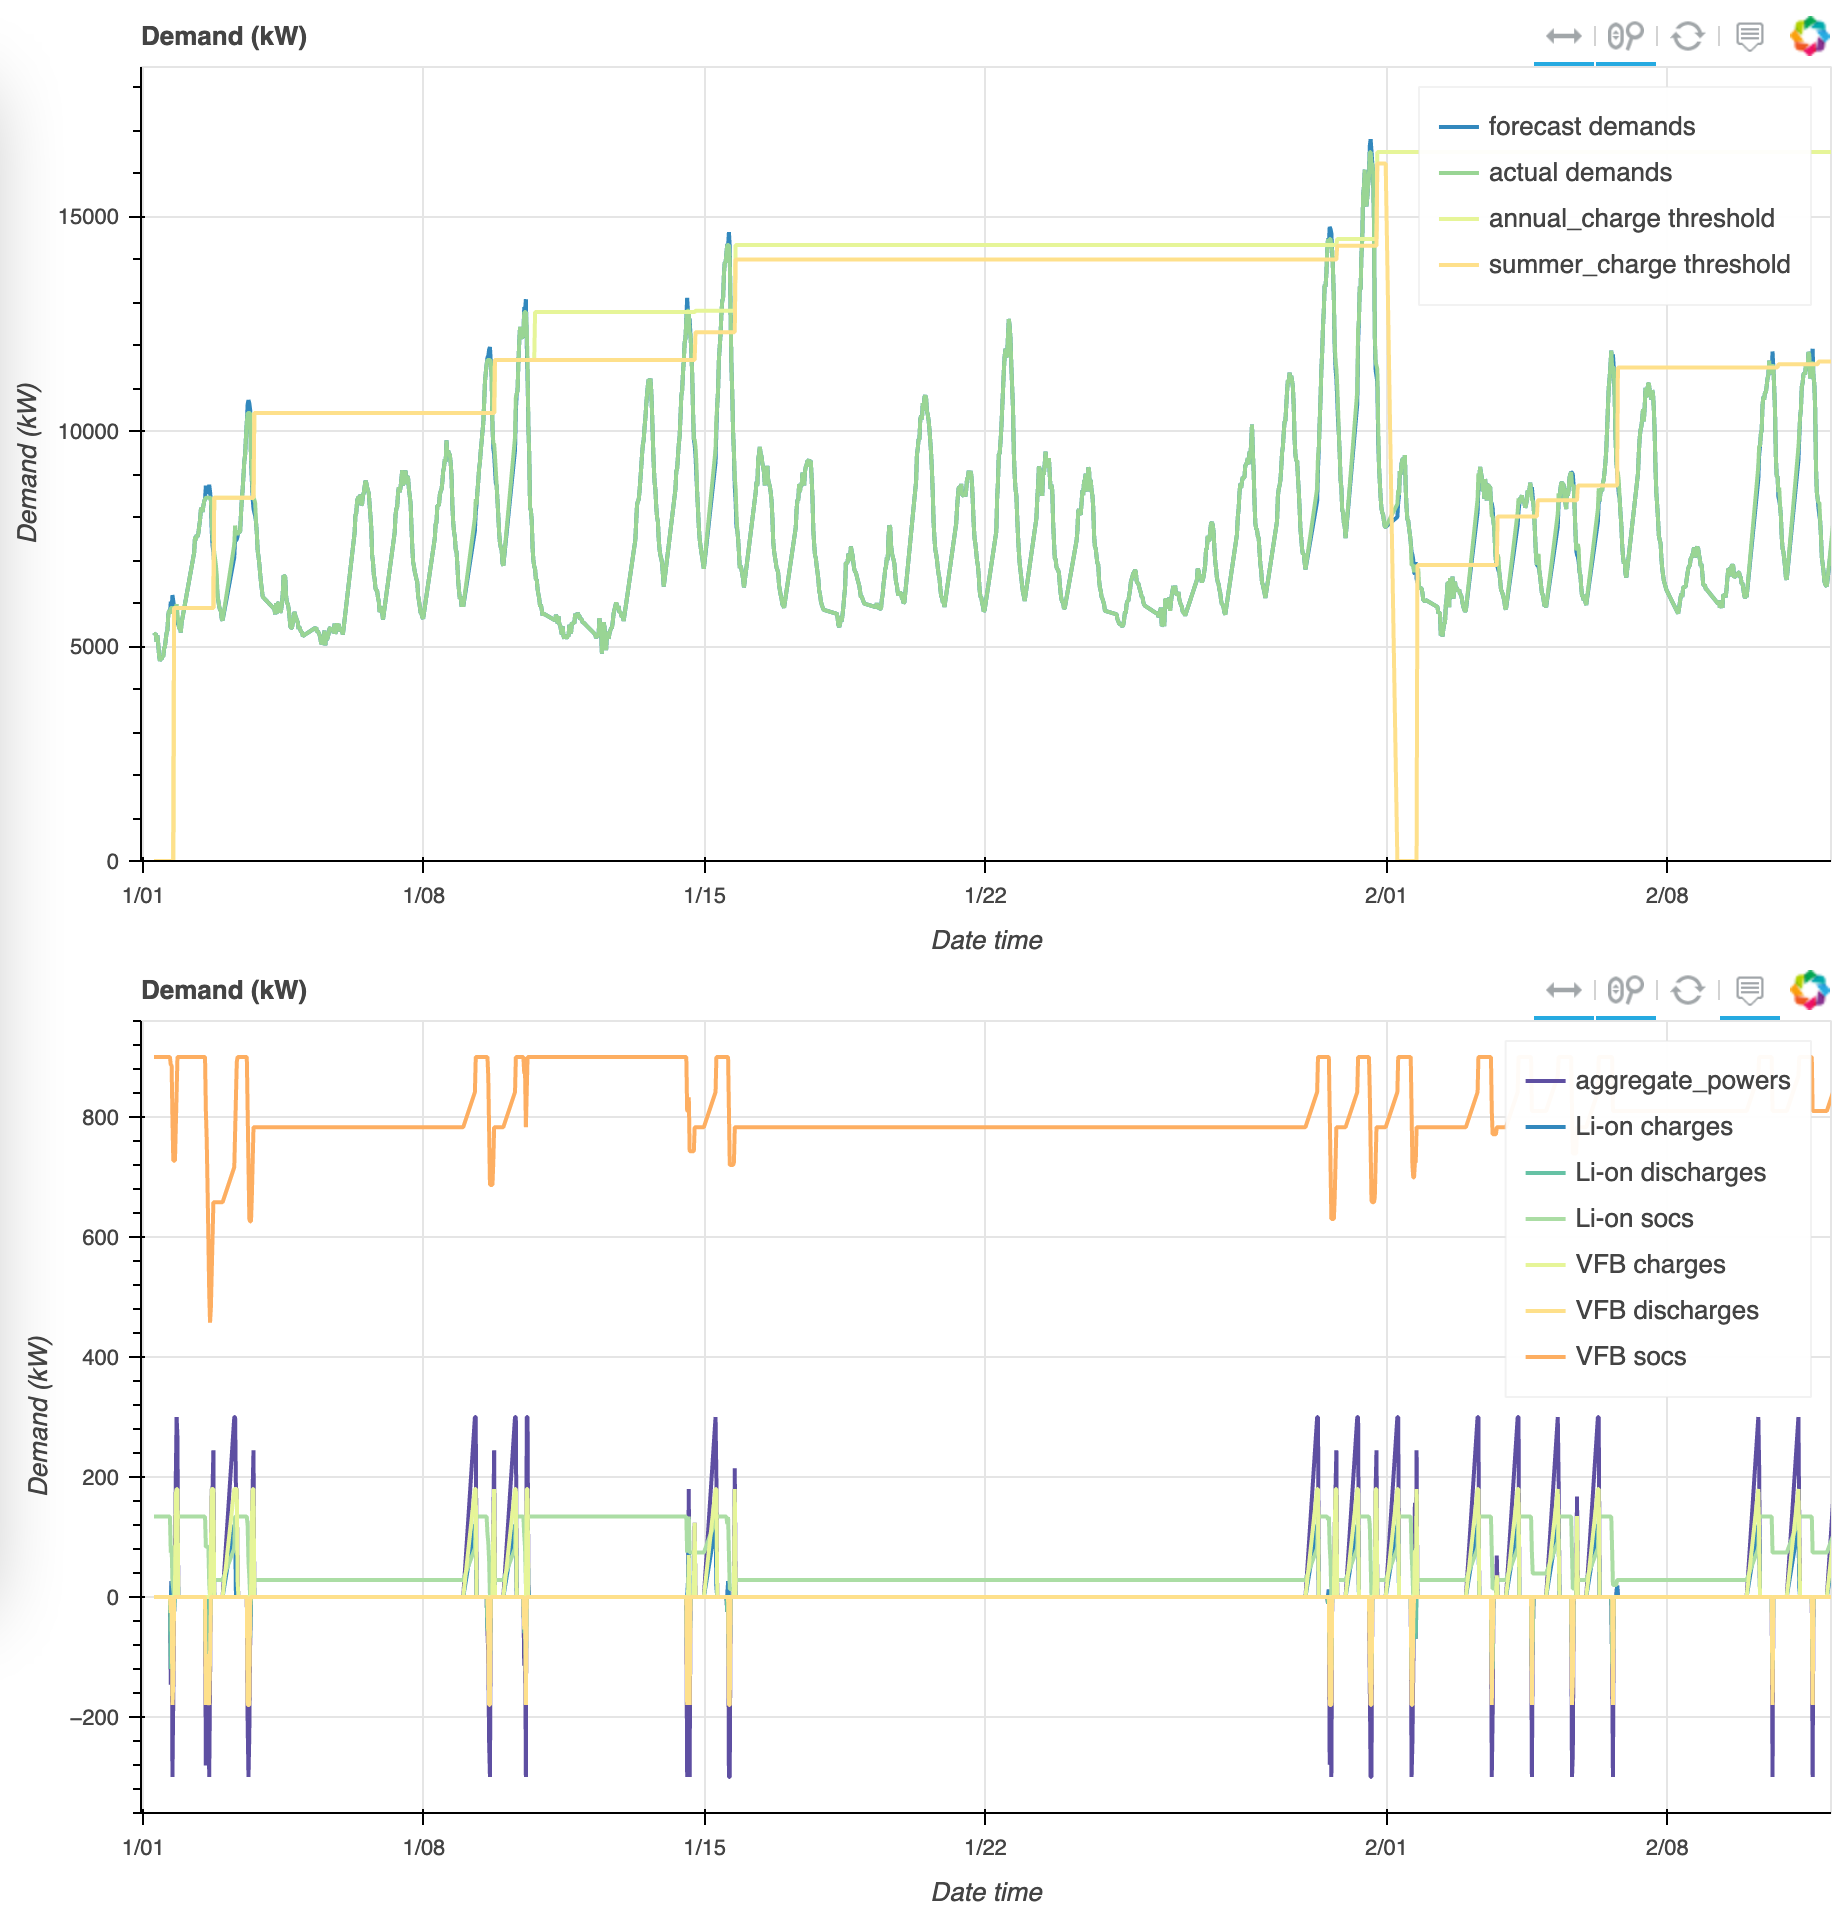
\includegraphics[width=1\linewidth]{pics/perfect-forecasts}
	\caption{Optimisation results with perfect forecasts}
	\label{fig:perfect-forecasts}
\end{figure}

\begin{figure}[p]
	\centering
	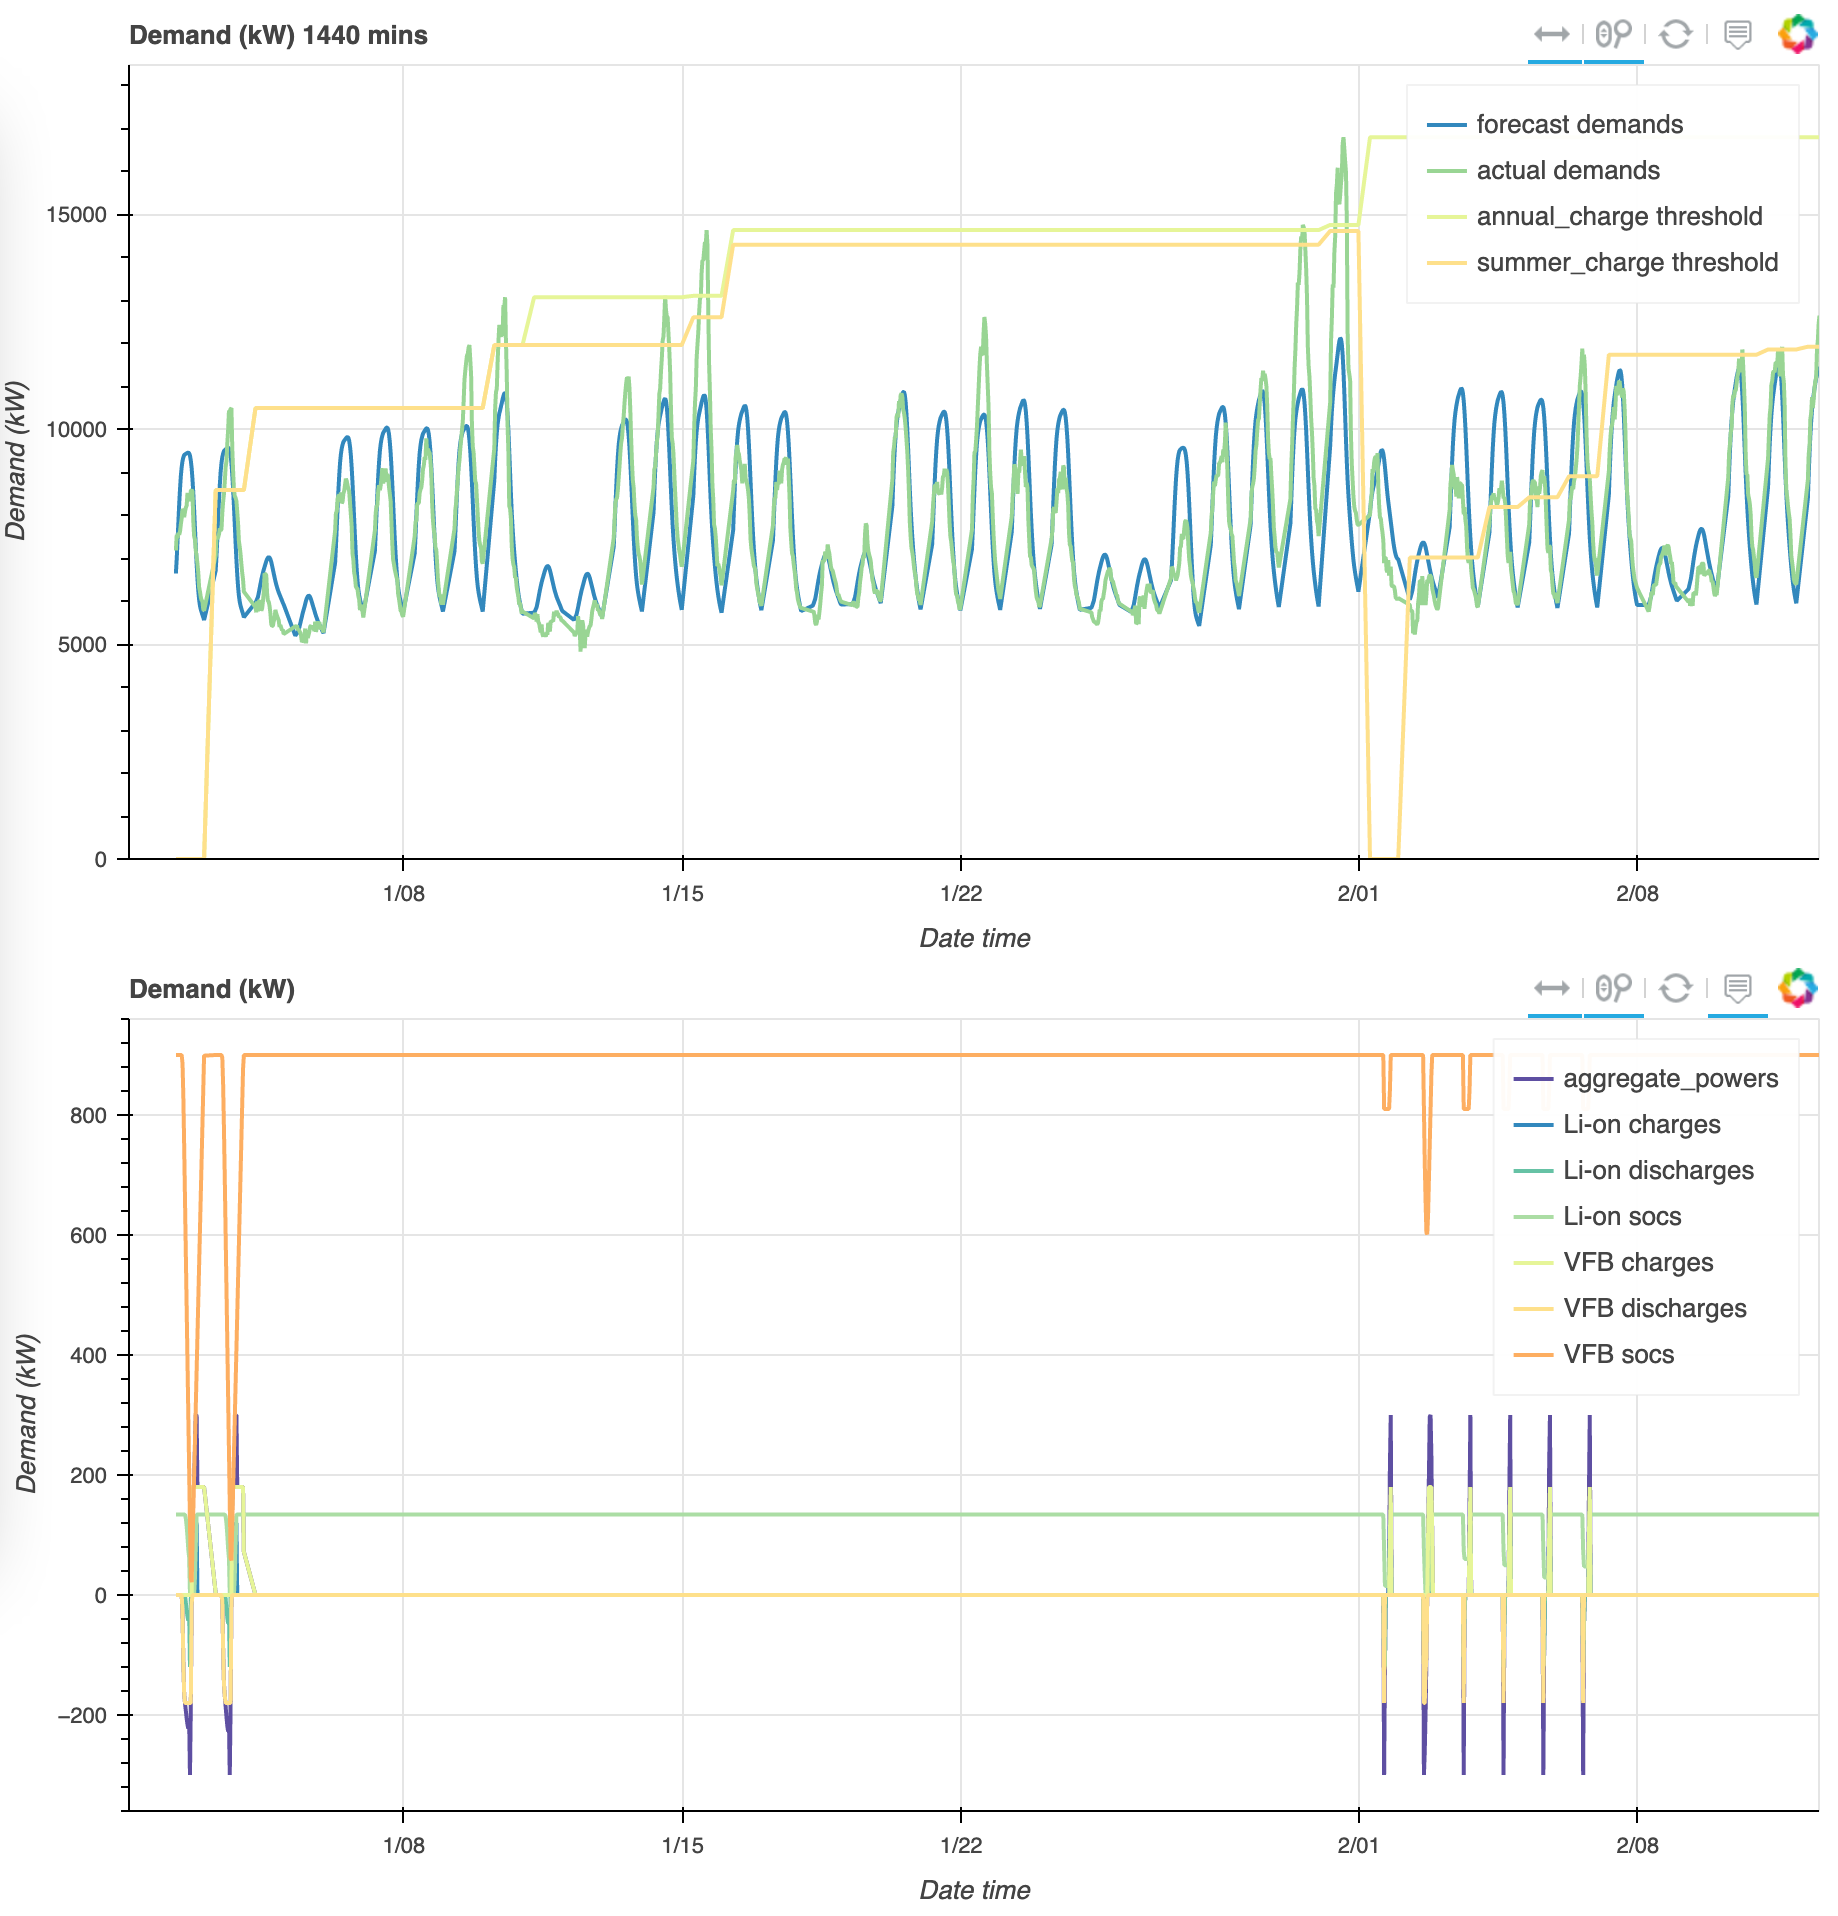
\includegraphics[width=1\linewidth]{pics/1440min-forecasts}
	\caption{Optimisation results with forecasts that are updated every day}
	\label{fig:1440min-forecasts}
\end{figure}

\begin{figure}[p]
	\centering
	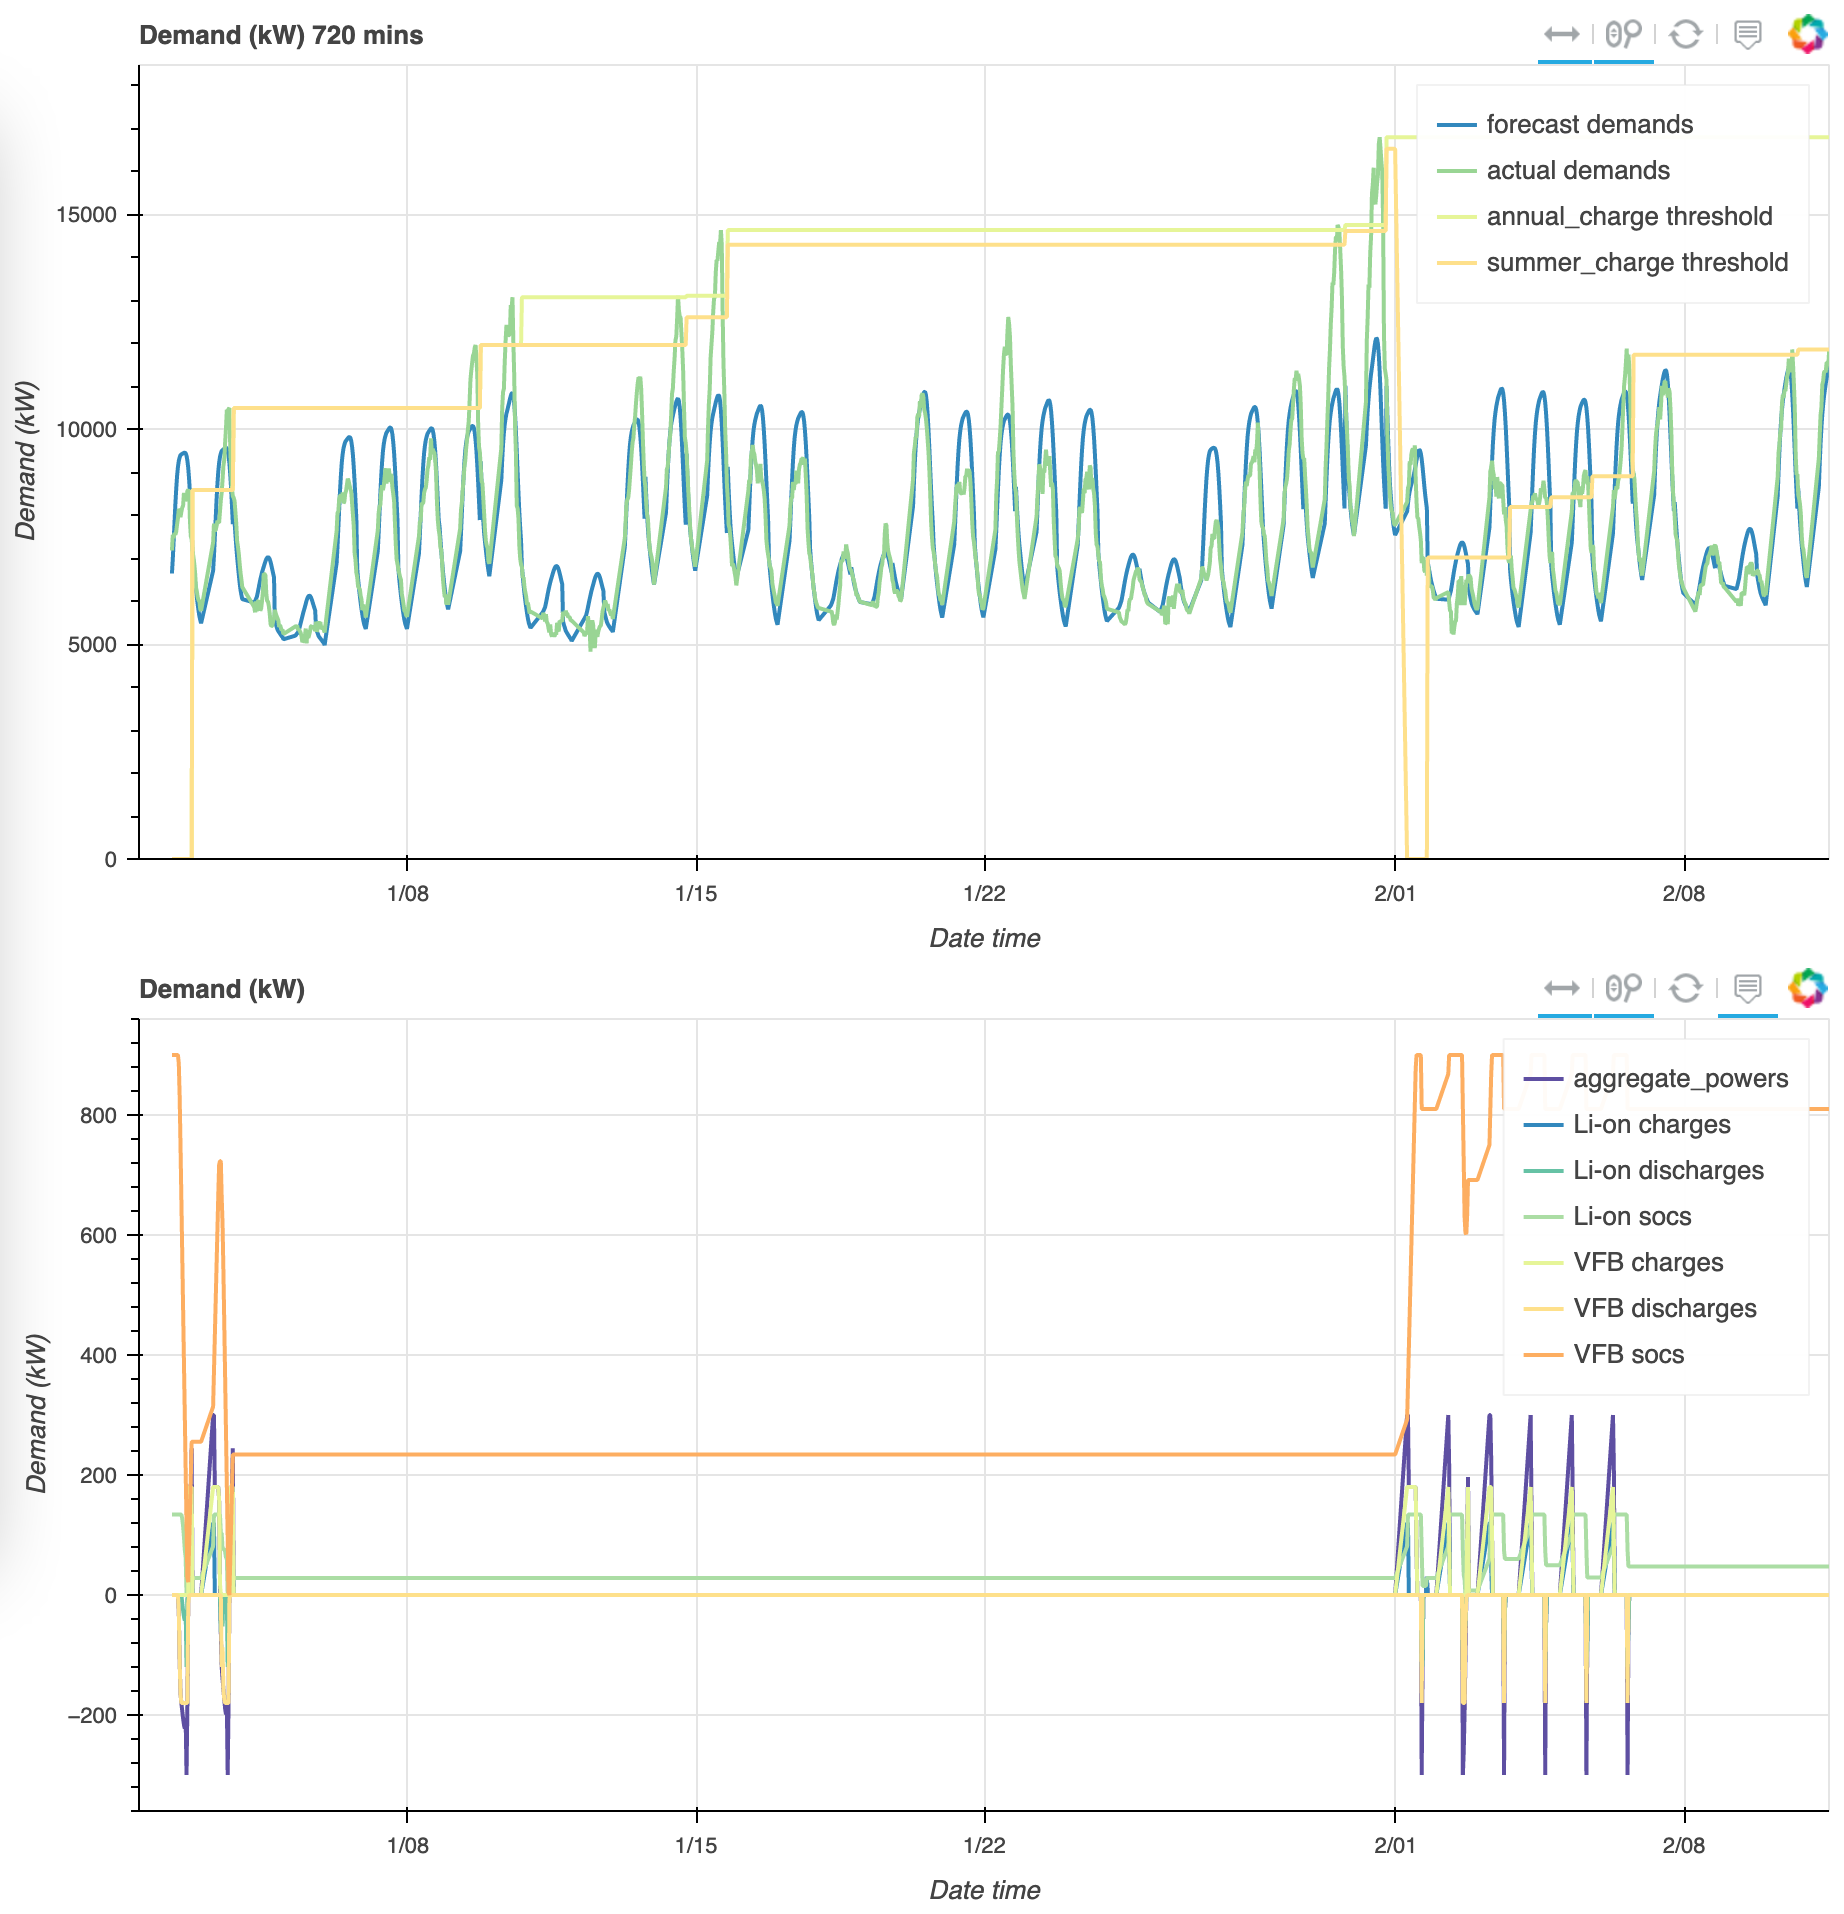
\includegraphics[width=1\linewidth]{pics/720min-forecasts}
	\caption{Optimisation results with forecasts that are updated every 12 hours}
	\label{fig:720min-forecasts}
\end{figure}

\begin{figure}[p]
	\centering
	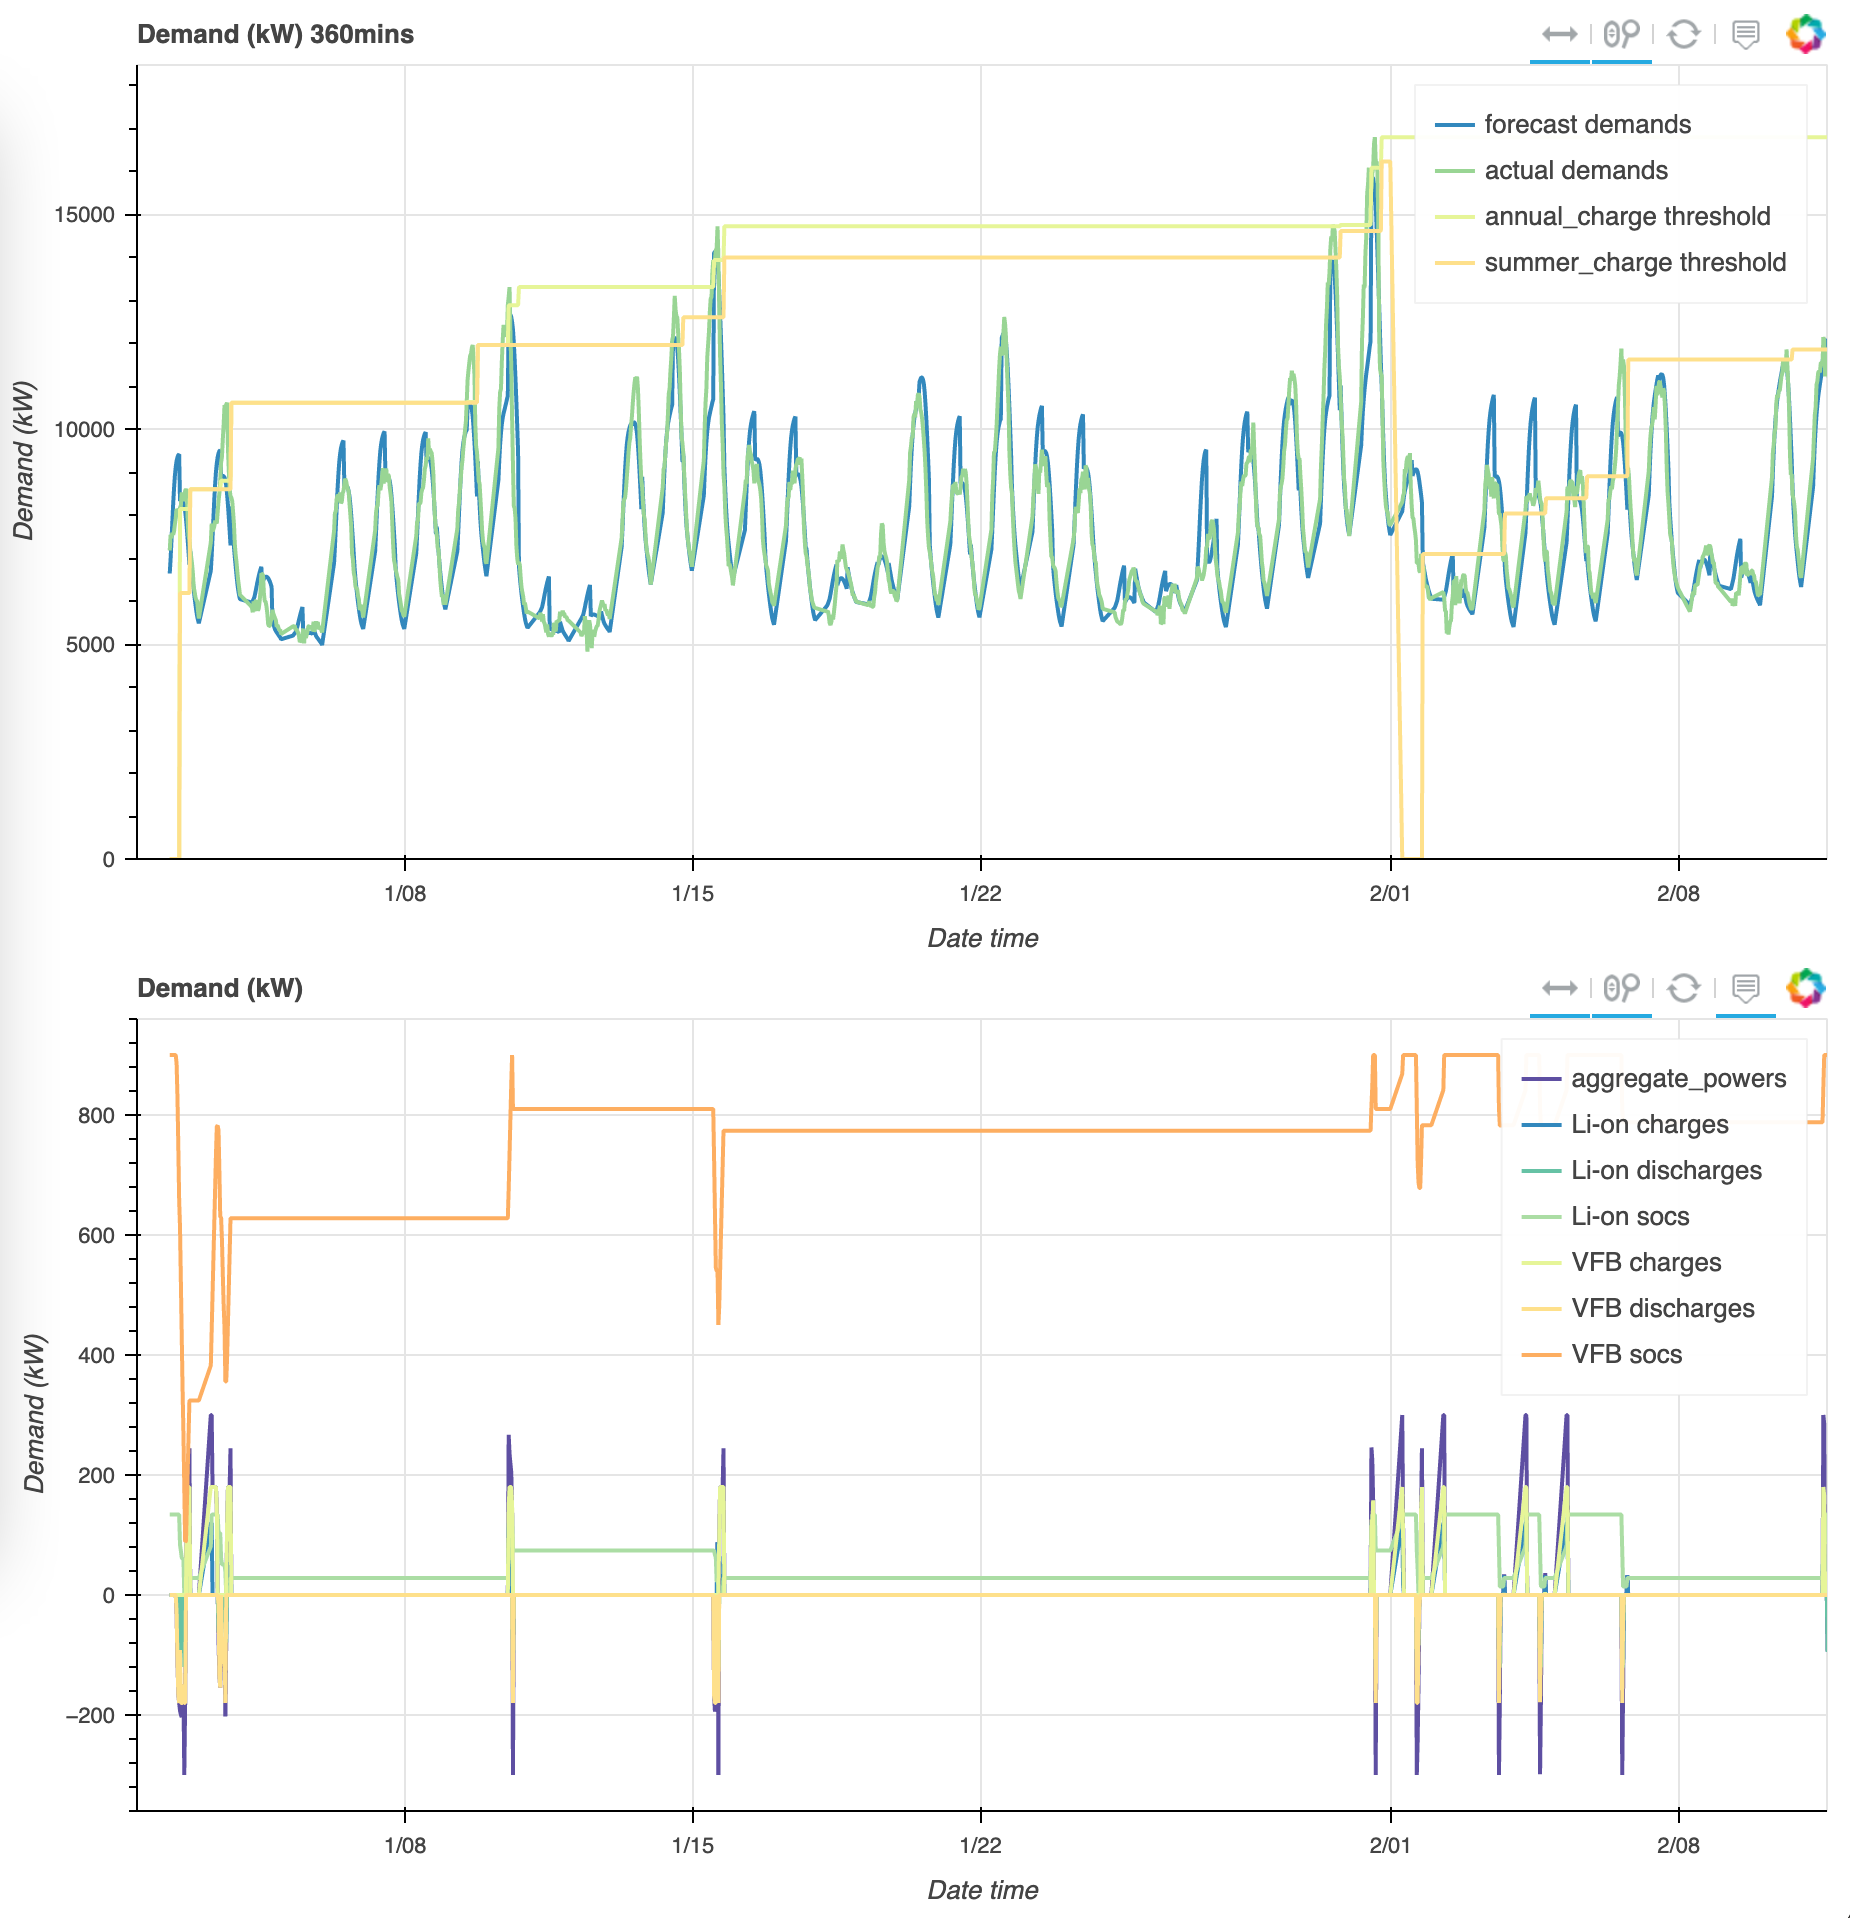
\includegraphics[width=1\linewidth]{pics/360min-forecasts}
	\caption{Optimisation results with forecasts that are updated every 6 hours}
	\label{fig:360min-forecasts}
\end{figure}

\begin{figure}[p]
	\centering
	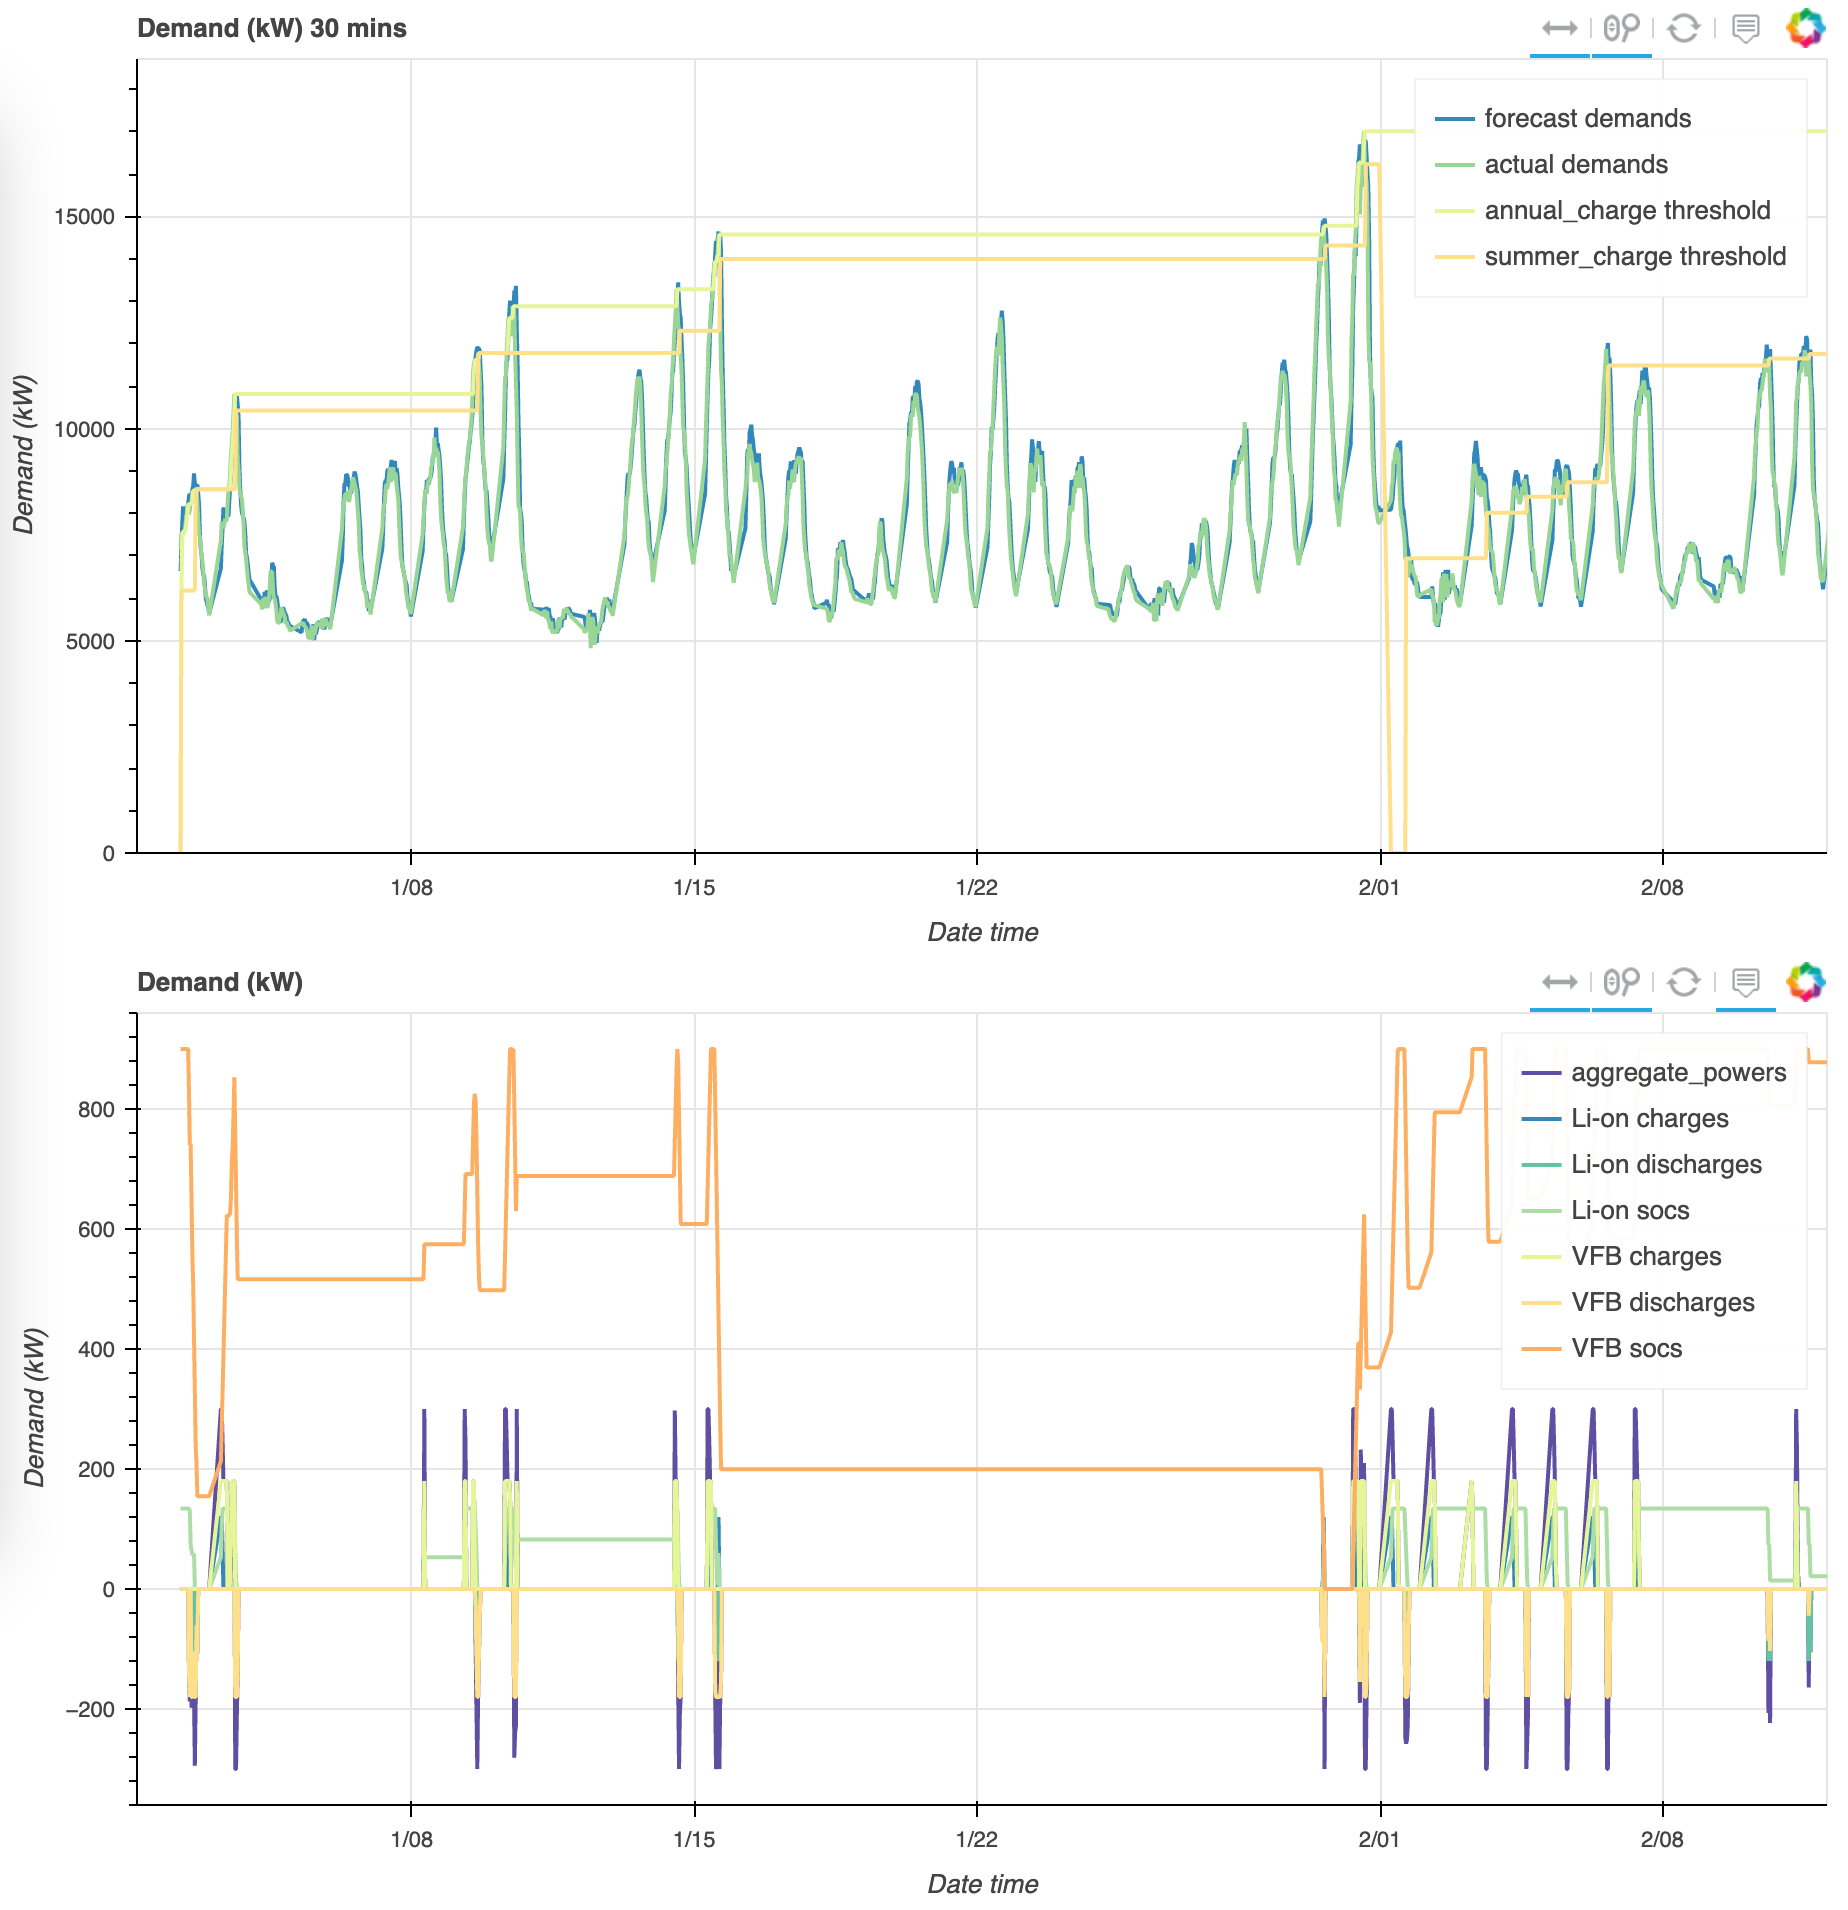
\includegraphics[width=1\linewidth]{pics/30min-forecasts}
	\caption{Optimisation results with forecasts that are updated every 30 minutes}
	\label{fig:30min-forecasts}
\end{figure}


\section{Conclusion}
\label{pdm:conclusion}

This work has developed a method that schedules batteries based on demand forecasts to reduce the \glsfirst{NPDC} for Monash Clayton campus. This method combines \glsfirst{LP} and \glsfirst{RHRS} to decide the best amount of power to charge and discharge for each battery at each time while incorporating uncertainty in the future demand. The experiment results have found that this method is effective at reducing the peak demand charges when the demand forecasts indeed approximate the actual demands. 

In order to hedge against the risks of uncertain future and inaccurate forecasts, future work can consider employing additional methods to incorporate various possible future scenarios, and scheduling batteries based on the expected outcomes of those future scenarios instead of a single forecast. Other future work can include investigating the scheduling results using different sizes of batteries, and evaluating the economic costs and returns of those battery sizes. 

